
\documentclass[journal]{IEEEtran}


\usepackage{hyperref}
\usepackage{amsmath}
\usepackage{amssymb}
\usepackage{hhline} % easy to manage table borders
\usepackage{colortbl} % colored cells in tables
\usepackage{multirow}
\usepackage{enumerate}
\usepackage{slashbox} % cell with slash inside
\usepackage{makeidx}  % allows index generation
\usepackage[utf8]{inputenc}
\usepackage{graphicx}
\usepackage{setspace}

\newtheorem{definition}{Definition}
\newtheorem{example}{Example}

\def\sectionautorefname{Section}
\def\subsectionautorefname{Section}


\begin{document}
%
% paper title
% can use linebreaks \\ within to get better formatting as desired
\title{Semantic Enrichment of E-Prescriptions using Linked Open Data}

\author{Ali~Khalili
        and~Bita~Sedaghati
\IEEEcompsocitemizethanks{\IEEEcompsocthanksitem A. Khalili is with the Institute of Informatics, University of Leipzig, Germany.
% note need leading \protect in front of \\ to get a newline within \thanks as
% \\ is fragile and will error, could use \hfil\break instead.
E-mail: khalili@informatik.uni-leipzig.de
\IEEEcompsocthanksitem B. Sedaghati is with Institute of Pharmacy, University of Leipzig, Germany.
E-mail: bita.sedaghati@uni-leipzig.de
}
}


% The paper headers
\markboth{International Journal On Advances in Life Sciences}%
{Khalili \MakeLowercase{\textit{et al.}}: Semantic Medical Prescriptions}
% The only time the second header will appear is for the odd numbered pages
% after the title page when using the twoside option.
%

% make the title area
\maketitle


\begin{abstract}
%\boldmath
The recent proliferation of Linked Open Data that enables the integration of multiple disparate data sources brings into the spotlight a new generation of knowledge management applications.
Particularly in the domain of pharmaceutical research and development, many efforts have been done to create a linked open drug data.
In this paper we present the Pharmer as an approach to facilitate the creation of semantic prescriptions.
Semantic prescriptions are intelligent e-prescription documents enriched by drug-related meta-data thereby know about their content and the possible interactions.
In an e-health system, semantic prescriptions provide an interoperable interface which helps patients, physicians, pharmacists, researchers and companies to collaboratively improve the quality of pharmaceutical services by facilitating the process of shared decision making.
Pharmer provides different views for the different personas involved in the process of e-prescribing.
It employs datasets such as DBpedia, DrugBank, DailyMed and RxNorm to automatically detect the drugs in the prescription and to collect multidimensional data on them.
Eventually it warns of the possible drug interactions in the prescription.
We evaluate the feasibility of the Pharmer by conducting a usability evaluation and report on the quantitative and qualitative results of our survey.
\end{abstract}


% Note that keywords are not normally used for peerreview papers.
\begin{IEEEkeywords}
 Semantic prescription, e-prescription, semantic annotation, e-health.
\end{IEEEkeywords}



\IEEEpeerreviewmaketitle


\section{Introduction}
\label{intro}

\section{LODD Applications}
\label{lod}

\section{Semantic Content Authoring}
\label{sca}


\section{Semantic E-Prescribing}
\label{sep}

\subsection{Architecture}

\subsection{Features}

\section{Pharmer as a Ubiquitous Computing Platform for Semantic E-Prescribing}
\label{mobile}

\begin{figure*}[tb]
 \centering
 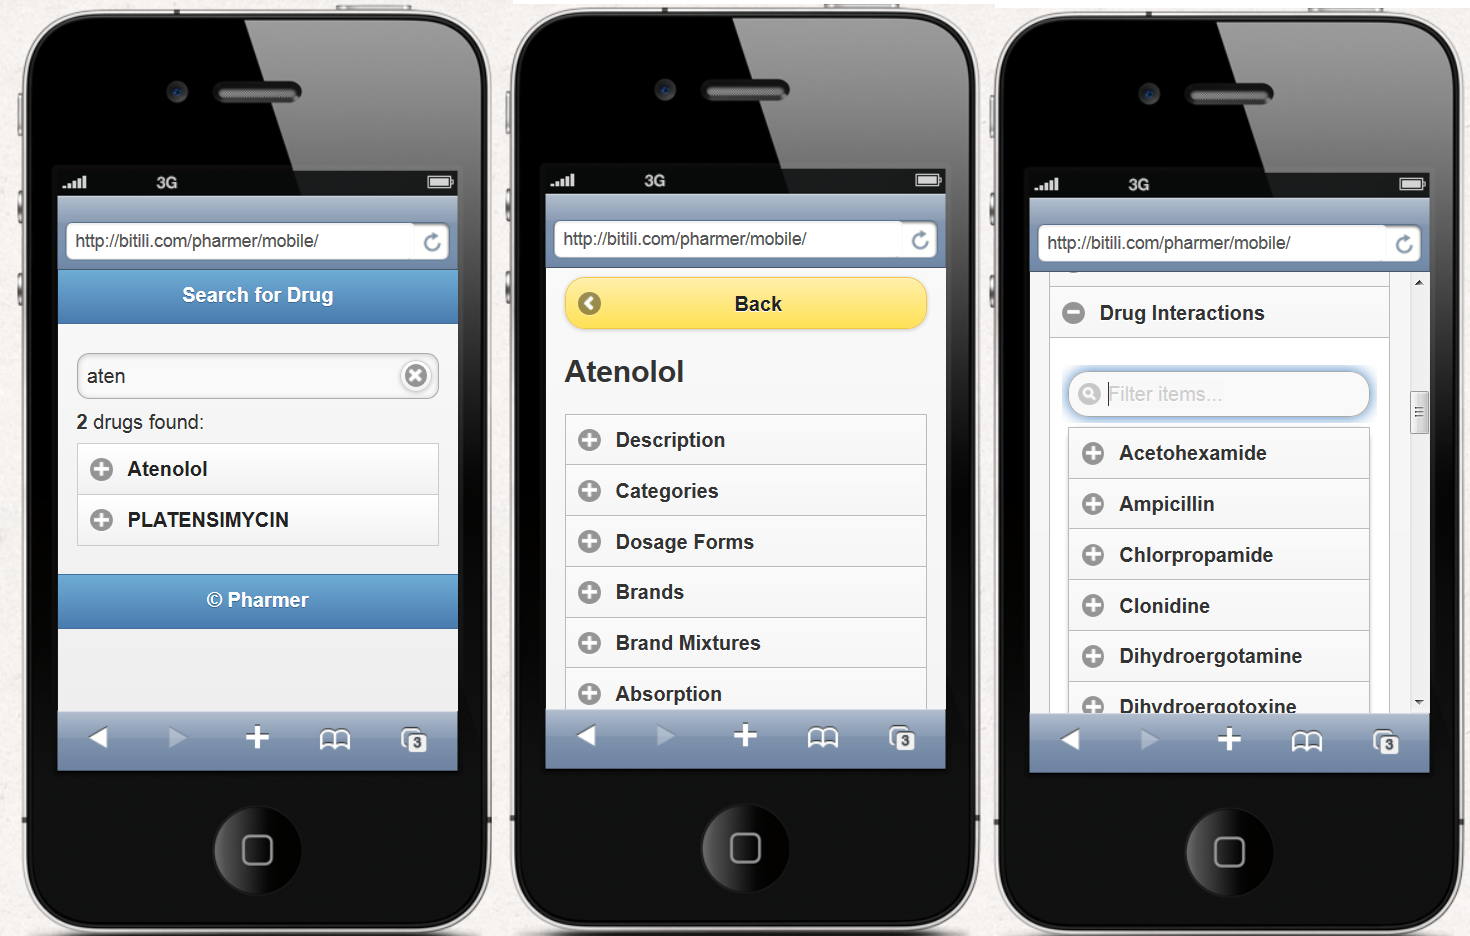
\includegraphics[width=1.5\columnwidth]{images/sc_pharmer.png}
	\caption{Screenshot of Pharmer Mobile Application (available at \url{http://bitili.com/pharmer/mobile}).}
 \label{fig:mobile}
\end{figure*}

Mobile and ubiquitous computing devices are increasingly present and prevalent in the health contexts.
This trend brings a number of possibilities of \emph{mobile health} (m-health) to address critical aspects of health care and health system needs, by virtue of these devices’ ubiquity, simplicity, and cost-efficiency~\cite{mHealth}.
In particular, in the process of semantic e-prescribing, having a mobile application will facilitate the creation of semantic medical prescriptions using any device and in any location.

Pharmer mobile application\footnote{ At the time of writing this paper, the Pharmer mobile application is still under development. The first beta version will be available on AppStore soon.} as shown in \autoref{fig:mobile} provides a mobile user interface for authoring of semantic prescriptions as well as accessing multi-dimensional data on medical prescriptions.
Current ubiquitous devices are programmable and come with a growing set of facilities including multi-touch screens and cheap powerful embedded sensors, such as an accelerometer, digital compass, gyroscope, GPS, microphone, camera and other type of sensors.
Utilizing these rich set of facilities in the context of medical prescriptions will enrich the patient medical prescription with sensor data thereby improves the quality of e-health services.

\section{Pharmer as a Professional Social Network for Health-care Service Providers}
\label{pharmernet}
\paragraph Pharmer offers couple of advantages over current e-prescribing systems:
The main benefit of using semantic prescriptions is the persistent connection to up-to-date drug information coming from multiple dynamic data sources.
So, when the information about a drug is updated occurs (e.g. change in its effects or interactions), the semantic prescription automatically adopts to this new change.

\paragraph Once writing a prescription it is very critical to consider drug interactions.
Drug interactions are divided to three categories namely \emph{food-drug}, \emph{drug-drug} and \emph{drug-plant} interactions.
Coadministration can either be synergistic or antagonistic which respectively increase or decrease the drugs effect.
The interactions may sometimes lead to change in the drug effect.
By applying semantic prescriptions, all types of drug interactions are prevented and the probability of errors in prescriptions are reduced to a great extend.

\paragraph A semantic prescription is a self-contained document which is aware of its content and is connected to the linked open data.
In contrast to database-oriented e-prescriptions, semantic prescriptions can easily be exchanged among other e-health systems without need to changing their related infrastructure hence enabling a connection between physicians, pharmacists, patients, pharmaceutical researchers, insurance and drug companies.

\paragraph Pharmer as a prescribing tool is able to be incorporated in a health care social network.
Such a network composed of health care professionals and patients who collaboratively write, correct and modify prescriptions in a semantically enriched environment.
This social health care network provides patients and health care providers with services. It further facilitates relations between paatients and health care professionals in order to improve shared decision making (SDM).
\paragraph 
As information source, the network access LODD, where diagnostic and prescribing data has been located. Accessing such pieces of information, Pharmer is able to be used as a tool for diagnosis and prescribing in assistance to physicians.
Privacy of that network is also a critical point worth considerations.
\subsection{Shared Decision Making}
\label{subsec: SDM}
\paragraph The traditional model of medical decision-making, in which doctors make decisions on treatment has no longer used in updated health care.The role of the patient, instead, in the consultation has been highlighted, mainly through introducing‘patient-centred’ strategies. Therefor, nowadays the models promoting patients active involvement in the decision-making procedure becoming developed.
 \paragraph A model introduced by Charles et al. defines shared decision making only under the following four key characteristics.
 These keys are:
 \begin{enumerate}
   \item both the patient and the doctor are involved
   \item both parties share information
   \item both parties take steps to build a consensus about the preferred treatment
   \item an agreement is reached on the treatment to implement
 \end{enumerate}

\paragraph Pharmer as social network facilitates shared decision making through the connection amongst patient and physician on one hand and pharmacist on the other hand. According to Charles et al. model, pharmer not only connects patients and physicians but also pharmacist as third party has an supervisory role on medication choice.

\subsection{Fast Diagnostic Tool}
\paragraph Free access to LODD enables Pharmer to not only linked to e-prescribing systems but also to further assist physicians in diagnosis and treatment. Pharmer with direct connection to up-to-date information enables doctors to reconfirm their diagnosis and help them in finding proper treatment approaches. Physician, after general examination, enters the observed symptoms in pharmer system and there, with the wealth of data available, pharmer assists in diagnosis followed by therapies.

\subsection{Privacy}
\paragraph Systems containing patient treatment history profiles, such as pharmer, required to be considered about privacy issues. This issue is solved by providing different users, with different views which is password protected. In such a protection, patient is only access his profile while physician has access to all of his patients, he same holds true for pharmacists and insurance companies. Other organisations(e.g. research institutes or pharma companies)can access to patients information as statistical data and only if the patient agrees. This protection helps pharmer users to ensure about data privacy.

\section{Example Scenario}
\label{es}

\section{Outlook}
\label{outlook}

\section{Conclusion}
\label{sec:conclusion}

\begin{spacing}{0.3}
\bibliographystyle{IEEEtran}
\bibliography{refs}
\end{spacing}

% that's all folks
\end{document}


